\section{Modelo}

A continuación veremos en detalle los distintos aspectos del problema a
 resolver, y como decidimos modelarlos para cumplir con los 
 requerimientos del problema. \\ \\
 
Se nos pide, en primer lugar, guardar para cada campeonato y cada 
categoria de dicho campeonato, todos los enfrentamientos con sus 
resultados y medallas. Podemos modelar esto de la siguiente manera:\\ \\

\begin{itemize}

\item En primer lugar tenemos una relacion $N,M$, entre los campeonatos y 
los arbitros que participaron en dicho campeonato. De la misma manera, 
existe una relación $N,M$ entre los competidores y un campeonato determinado, 
y las escuelas y un campeonato.\\

\item El campeonato debe estar relacionado con la entidad enfrentamientos.
Como cada enfrentamiento esta directamente asociado a una categoria y a 
un campeonato, entonces podemos modelar una relacion 1 a 1 entre enfrentamiento
y su modalidad; y una relacion 1 a N entre el campeonato y sus enfrentamientos.\\

\item Por último, los campeonatos deben conocer los medalleros correspondientes a 
cada categoria. Luego necesariamente debemos modelarlo como una relacion 
$N,M$ entre el medallero y el campeonato.\\

\end{itemize}

Además de cumplir con los requerimientos básicos del enunciado, debemos asegurarnos 
de modelar el problema de tal manera que las consultas puedan resolverse 
eficientemente. \\

Algunas relaciones triviales que se desprenden de las consultas son: 
los enfrentamientos estan relacionados con competidores; las escuelas están 
relacionadas con competidores. \\ \\

Luego el Diagrama de entidad relacion para este problema es:


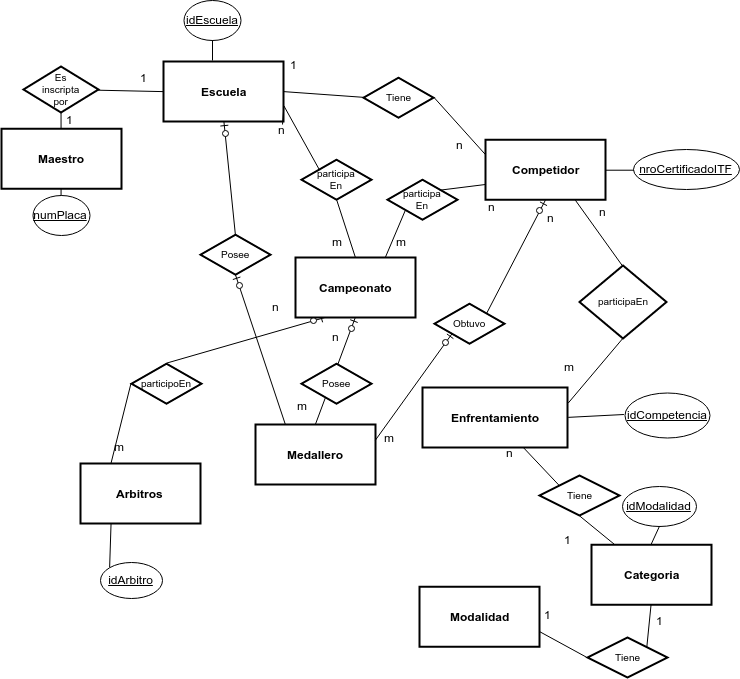
\includegraphics[scale=0.55]{diagDer.png}
 
 Un aspecto a tener en cuenta es que a diferencia del TP1, como tenemos 
 datos historicos. los datos de peso graduacion y edad no se van a corresponder
 con las restricciones  de cada compentencia. Es decir, podria llegar a tener a 
 un competido de 40 años, pero en su historial figura que compitio en una categoria
 de hasta 30 años. Lo Cual tiene sentido si dicha competencia ocurrior con 
 bastante más anterioridad.\\
